% IMPORTANT: PLEASE USE XeLaTeX FOR TYPESETTING
\documentclass[10pt]{beamer}

\usetheme{Darmstadt}%{default}
\usecolortheme{beaver}
\usepackage[T1]{fontenc} 
\usepackage[utf8]{inputenc}
\usepackage[french]{babel}
\usefonttheme{serif}
\usepackage{lmodern}
\usepackage{tcolorbox}
 % pour un pdf lisible à l'écran
 % il y a d'autres choix possibles 
\usepackage{pslatex}
% \usepackage{ctex, hyperref}
\usepackage{latexsym,amsmath,xcolor,multicol,booktabs,calligra}
\usepackage{graphicx,pstricks,listings,stackengine}
\usepackage{chemfig}

\usepackage{tabularx}
% meta-data
\title{Leçon :Effet tunnel, radioactivité $\alpha$}

\author{Gabriel Le Doudic}
\institute{Préparation à l'agrégation de Rennes}
% \titlebackground{images/background}

\definecolor{aquamarine}{rgb}{0.5, 1.0, 0.83}
\definecolor{applegreen}{rgb}{0.55, 0.71, 0.0}	
\definecolor{cobalt}{rgb}{0.0, 0.28, 0.67}

\definecolor{definitionf}{RGB}{220,252,220}
\definecolor{definitionl}{RGB}{39,123,69}
\definecolor{definitiono}{RGB}{72,148,101}

\definecolor{propositionf}{RGB}{255,216,218}
\definecolor{propositionl}{RGB}{38,38,38}
\definecolor{propositiono}{RGB}{109,109,109}

\definecolor{theof}{RGB}{255,216,218}
\definecolor{theol}{RGB}{160,0,4}
\definecolor{theoo}{RGB}{221,65,100}

\definecolor{avertl}{RGB}{163,92,0}
\definecolor{averto}{RGB}{255,144,0}

\definecolor{histf}{RGB}{241,238,193}

\definecolor{metf}{RGB}{220,230,240}
\definecolor{metl}{RGB}{56,110,165}
\definecolor{meto}{RGB}{109,109,109}


\definecolor{remf}{RGB}{230,240,250}
\definecolor{remo}{RGB}{150,150,150}

\definecolor{exef}{RGB}{240,240,240}

\definecolor{protf}{RGB}{247,228,255}
\definecolor{protl}{RGB}{105,0,203}
\definecolor{proto}{RGB}{174,88,255}

\definecolor{grid}{RGB}{180,180,180}

\definecolor{titref}{RGB}{230,230,230}

\definecolor{vert}{RGB}{23,200,23}

\definecolor{violet}{RGB}{180,0,200}

\definecolor{copper}{RGB}{217, 144, 88}
%% CADRES

\newtcolorbox{defi}[1]{
	colback=applegreen!5!white,
  	colframe=applegreen!65!black,
	fonttitle=\bfseries,
  	title={#1}}
\newtcolorbox{Programme}[1]{
	colback=cobalt!5!white,
  	colframe=cobalt!65!black,
	fonttitle=\bfseries,
  	title={#1}}  
\newtcolorbox{Resultat}[1]{
	colback=theof,%!5!white,
	colframe=theoo!85!black,
  fonttitle=\bfseries,
	title={#1}} 
\usepackage{tikz}
\usepackage{array}
\usepackage[scientific-notation=true]{siunitx}
\usetikzlibrary{matrix}
\newcommand{\diff}{\mathrm{d}}

\title{Leçon : Mécanisme de la conduction électrique dans les solides}

% document body
\begin{document}
\begin{frame}{}
    \titlepage

    \begin{tabularx}{\textwidth}{l@{:\,\,}X}
        \textbf{Niveau} 	  & CPGE deuxième année\\
        \textbf{Prérequis} & Électronicétique \\
        & Électromagnétisme \\
        & équations de Maxwell \\
        & Théorie cinétique des gaz
        
    \end{tabularx}
\end{frame}

\begin{frame}
    \tableofcontents
\end{frame}


\section{Modèle de Drude}
\section{Vision quantique de la conduction électrique}
\subsection{Distribution de Fermi Dirac}
\begin{frame}{Gaz d'électrons libres 1D}
\begin{minipage}{.45\textwidth}
    \centering
    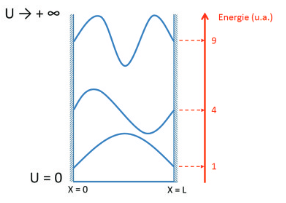
\includegraphics[width=1\textwidth]{Gaz1D.png}
\end{minipage}
\begin{minipage}{.45\textwidth}
    \begin{equation}
        \begin{array}{cc}
        -\dfrac{\hbar^2}{2m}\Delta\psi(x)=\epsilon\psi(x) & \text{ pour } 0 \geq x\geq L.
        \end{array}
    \end{equation}
    Solution : 
    \begin{equation}
        \psi(x)=\sqrt{\dfrac{2}{L}}\sin(k_x x)
    \end{equation}

    \begin{equation}
        \begin{array}{ccc}
        \epsilon=\dfrac{\hbar^2k_x^2}{2m}, & k_x=n_x\dfrac{\pi}{L}, & n_x \text{ entier } >0.
        \end{array}
    \end{equation}
\end{minipage}
\pause
Densité d'états dans l'espace des $k$ et d'énergie:
\begin{equation}
    \begin{array}{cc}
    g(k_x)=\dfrac{L}{\pi}\times 2 (\uparrow\downarrow), &  g(\epsilon)=L\dfrac{\sqrt{2m}}{\hbar\pi}\dfrac{1}{\sqrt{\epsilon}}.
    \end{array}
\end{equation}
\end{frame}

\begin{frame}{Gaz d'électrons libres 3D}
    Solution: 
    \begin{equation}
        \begin{array}{cc}
        \psi(x,y,z) = \sqrt{\dfrac{8}{V}}\sin(k_x x)\sin(k_y y)\sin(k_z z), & \epsilon = \dfrac{\hbar^2\vec{k}^2}{2m}
        \end{array}
    \end{equation}
Chaque solution est repérée par un vecteur d'onde $\vec{k} = \left(k_x=n_x\frac{pi}{Lx}, k_y=n_y\frac{\pi}{Ly}, k_z=n_z\frac{\pi}{Lz}\right)$.
\pause

Densité d'états dans l'espace des $\vec{k}$

\begin{equation}
    g(\vec{k})d^3\vec{k}=\dfrac{d^3\vec{k}}{\frac{\pi}{L_x}\frac{\pi}{L_y}\frac{\pi}{L_z}}\times 2 (\uparrow\downarrow) = \dfrac{2V}{pi^3}d^3\vec{k}\rightarrow g(\vec{k})=\dfrac{V}{\pi^3}\times 2(\uparrow\downarrow)
\end{equation}


Densité d'états en énergie
\[g(\epsilon)d\epsilon=g(\vec{k})dV_{k}=g(\vec{k})4\pi k^2dk\times \dfrac{1}{8}\]
Soit : 
\begin{equation}
g(\epsilon) = \dfrac{V}{2\pi^2}\left(\dfrac{2m}{\hbar^2}\right)^{3/2}\epsilon^{1/2}.    
\end{equation}
\end{frame}

\subsection{Comment relier ce modèle à la conductivité électrique}
\begin{frame}{\insertsubsection}
    \begin{figure}
        \centering
        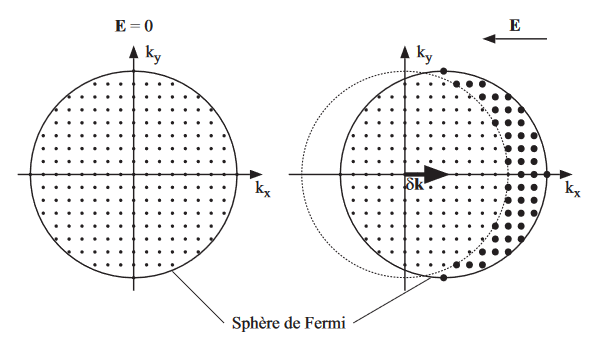
\includegraphics[width=.7\textwidth]{SphereDeFermi.png}
    \end{figure}
\end{frame}
\section{Matériaux isolants/ conducteurs/ semi-conducteurs}

\subsection{Théorie des bandes}

\begin{frame}{Théorie des bandes}
    \begin{figure}
        \centering
        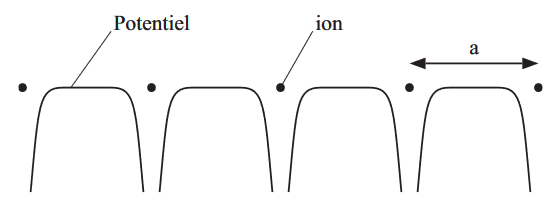
\includegraphics[width=.7\textwidth]{PotentielPeriodique.png}
    \end{figure}
\end{frame}

\subsection{Isolant, conducteur}
\begin{frame}{\insertsubsection}
    \begin{figure}
        \centering
        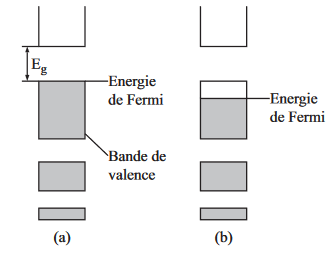
\includegraphics[width=.7\textwidth]{Isolant-conducteur.png}
    \end{figure}
\end{frame}
\end{document}